%
% Simple asymmetric two-column CV 
% Author: Sofia JIJON
%

\documentclass[a4paper,10pt]{article}
\usepackage[vmargin=1.5cm, hmargin=1.0cm]{geometry}
\usepackage{setspace}
% !TEX root = Simple-CV.tex
%-------------------------------------------------------------------------------------------------------
% Packages
%-------------------------------------------------------------------------------------------------------
\usepackage[english]{babel}
\usepackage[utf8]{inputenc}
\usepackage{fontawesome}
\usepackage{datetime}
\usepackage[usenames,dvipsnames]{xcolor}
\usepackage[colorlinks=true, urlcolor=ColorTwo]{hyperref}
\usepackage{tikz}
\usepackage{hyperref}
\usepackage{setspace}
\usepackage{graphicx}
\usepackage{enumitem}
\usepackage{sectsty}
\usepackage{multicol}
\usepackage{adjustbox}
%-------------------------------------------------------------------------------------------------------
% Layout
%-------------------------------------------------------------------------------------------------------
\pagenumbering{gobble}
\renewcommand{\baselinestretch}{1.5} 
\setlength{\parindent}{0pt}

%
% Color theme
%
\definecolor{ColorOne}{RGB}{0,0,0} 	% Blue
\definecolor{ColorTwo}{RGB}{106,106,106} 	% Mauve
%\definecolor{ColorTwo}{RGB}{140,100,0} 	% Gold

\sectionfont{\color{ColorOne}} 
\subsectionfont{\color{ColorOne}} 

%
% Vertical line
%
\newcommand{\MyVerticalRule}{%
	\textcolor{ColorOne}{\rule{1pt}{\textheight}}
}

%
% Update
%
\newcommand{\LastUpdate}{%
\vfill
\centering \small
\textcolor{ColorOne}{Last updated: \monthname,~\the\year }
}

%
% Skip
%
\newcommand{\MySkip}{
\vskip12pt
}

%
% Format hyperrefs
%
\newcommand{\myhref}[2]{%
\href{#1}{\textcolor{ColorTwo}{#2}}
}
%
% Format skill bullets
%
\newcommand{\SkillBull}[1]{%
\textcolor{ColorTwo}{#1}
}


%-------------------------------------------------------------------------------------------------------

\begin{document}
%-------------------------------------------------------------------------------------------------------
% Left column
%-------------------------------------------------------------------------------------------------------
\begin{adjustbox}{valign=t}
\begin{minipage}{0.3\textwidth} % Adapt width to your convenience
%----------------------------------------------------
% Please add a photo in 1x1 format
\begin{center}
\begin{tikzpicture}
	\clip (0,0) circle (2cm) node {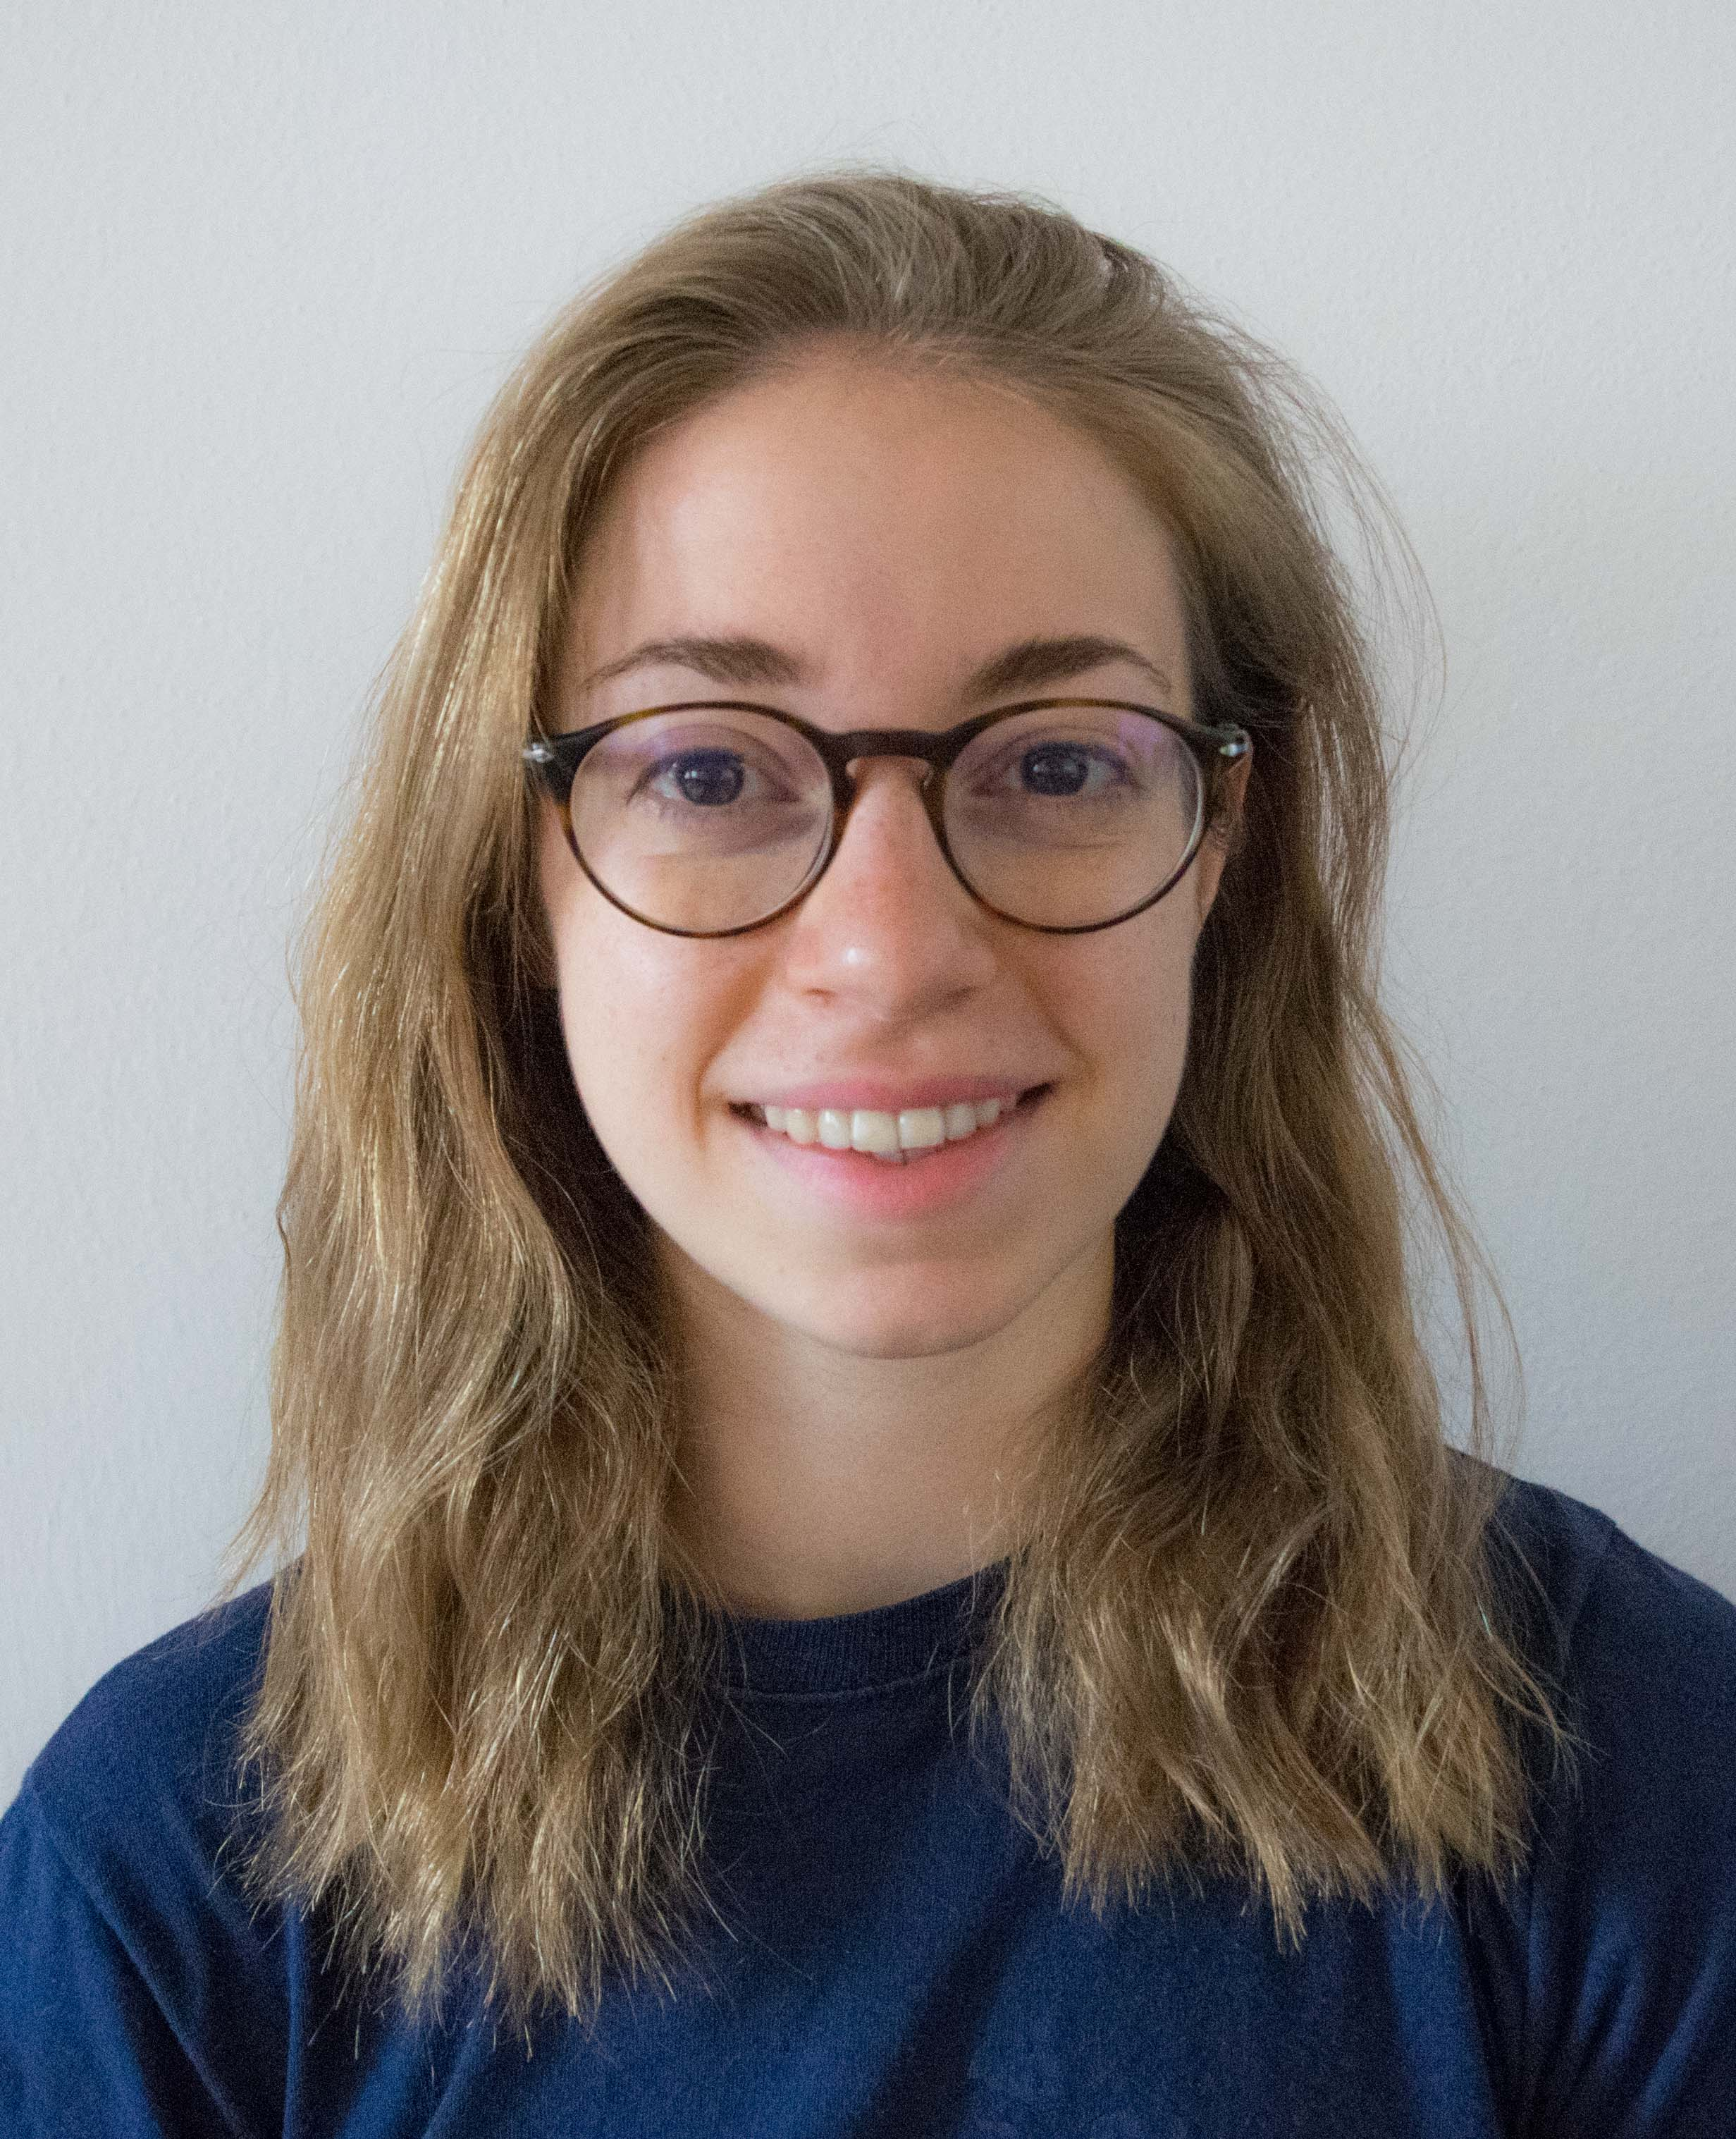
\includegraphics[width=4cm]{propic}};
\end{tikzpicture}

\MySkip 	% See MySetup.tex file

%----------------------------------------------------
{\LARGE \bfseries Elena Acinapura}

\MySkip 	% See MySetup.tex file

Born in Bolzano, Italy, 1999\\
Living in Zürich, Switzerland\\

\MySkip 	% See MySetup.tex file

\textcolor{ColorTwo}{\faEnvelopeO} 
\myhref{mailto:elena.acinapura@gmail.com}{elena.acinapura@gmail.com} \\

\textcolor{ColorTwo}{\faChain} 
\myhref{https://elena.acinapura.it}{elena.acinapura.it}
\end{center}

\vfill

%----------------------------------------------------
\section*{Scientific interests}
\raggedright
\textcolor{ColorOne}{$\circ$} Quantum computing\\
\textcolor{ColorOne}{$\circ$} Experimental physics\\
\textcolor{ColorOne}{$\circ$} Computational physics\\

\vfill

%----------------------------------------------------
\section*{Education}
	\begin{description}
	\raggedright
	\item []\normalfont \textcolor{ColorTwo}{2021 - Now}\\
    \textbf{MSc. in Quantum Engineering}\\
	ETH Zürich\\
	Zürich -- Switzerland

	\item []\normalfont \textcolor{ColorTwo}{2018 - 2021}\\ \textbf{BSc. in
	Physics}\\
	University of Trento\\
	Trento -- Italy\\
    \small{Graduated with 110/110 cum laude}
    \normalsize

	\item []\normalfont \textcolor{ColorTwo}{2013 - 2018}\\
	\textbf{Secondary School}\\ 
	Liceo Classico \textit{"G. Carducci"} \\
	Bolzano -- Italy \\
    \small{Concluded with 100/100 cum laude} \normalsize
\end{description}

% \vfill
\end{minipage}
\end{adjustbox}
%
%
%-------------------------------------------------------------------------------------------------------
% Vertical rule
%-------------------------------------------------------------------------------------------------------
%
\hfill
\begin{adjustbox}{valign=t}
\begin{minipage}{0.05\textwidth} % Adapt width to your convenience
\MyVerticalRule  % See MySetup.tex file
\end{minipage}
\end{adjustbox}
% \hfill
%
%-------------------------------------------------------------------------------------------------------
% Right column
%-------------------------------------------------------------------------------------------------------
\begin{adjustbox}{valign=t}
\begin{minipage}{0.6\textwidth} % Adapt width to your convienience

%----------------------------------------------------
\section*{Working Experience}
\begin{description}
\setlength\itemsep{-1em}
\item[\normalfont \textcolor{ColorTwo}{mar. 2022 -- Present}] 
	\textbf{Semester Project at QuDev}\\
	\emph{ETH Zurich, Supervisor: Prof.\ Dr.\ Andreas Wallraff}
	\begin{spacing}{1.1}
		\small
	I am working in the Hybrid Team with the goal of measuring the coupling between a transmon and a double quantum dot.
	\end{spacing}
\item[\normalfont \textcolor{ColorTwo}{Sep. 2022 -- Mar. 2023.}] 
	\textbf{Internship at Zurich Instruments}\\
	\emph{Zurich Instruments}
	\begin{spacing}{1.1}
		\small
	I worked on enabling automated system testing of the python software controlling the Zürich Instruments devices. Additionally, I extended the testing capabilities by performing complex quantum experiments such as Repeat-Until-Success and Bell State Stabilization.
	\end{spacing}
\item[\normalfont \textcolor{ColorTwo}{Jul. 2022 -- Aug. 2022.}] 
	\textbf{Research assistant at the Photonic Lab}\\
	\emph{ETH Zurich, Supervisor: Prof.\ Dr.\ Lukas Novotny}
	\begin{spacing}{1.1}
		\small
	I continued the activities started in my semester project (see below), working on further improving the setup and solving noise-to-ratio related issues.
	\end{spacing}
\item[\normalfont \textcolor{ColorTwo}{Mar. 2022 -- Jun. 2022.}] 
	\textbf{Semester project at the Photonic Lab}\\
	\emph{ETH Zurich, Supervisor: Prof.\ Dr.\ Lukas Novotny}
	\begin{spacing}{1.2}
		\small
	I worked on the generation of a bistable trap with optical tweezers and studied the stochastic motion of a dielectric nanoparticle trapped in the bistable potential.
	\end{spacing}
\end{description}
%----------------------------------------------------
\vspace{-1cm}
\section*{Knowledge and Technical Skills}
\begin{description}
\setlength\itemsep{-2em}

\item \textbf{Quantum Information Processing}
\begin{spacing}{1.1}
	\small Solid knowledge of the foundations of quantum optics, quantum algorithms, quantum error correction, superconducting circuits, ion traps, quantum dots and spin qubits.
\end{spacing}
\item \textbf{Experimental Physics}
\begin{spacing}{1.1}
	\small Experience on \textbf{optical setups}, lasers and photo detection. I am also gaining experience with \textbf{electronic measurements} for superconducting qubits and semiconducting devices in \textbf{cryogenic setups}. I feel at ease with common instruments for electronic measurements such as oscilloscopes and multimeters.
\end{spacing}
\item \textbf{Computer Science}
\begin{spacing}{1.1}
	\small
	Experienced in algorithms, data structures and testing engineering.\\
	My main programming languages are \textbf{Python} (object-oriented programming, data analysis for scientific experiments, test engineering with pytest) and \textbf{C/C++} (experience from the development of a library for computational physics as a personal project and from algorithmic programming).
\end{spacing}
\end{description}
%----------------------------------------------------
\vspace{-1cm}
\section*{Further Experiences}
\begin{description}
\raggedright
\setlength\itemsep{-1em}
\item[\normalfont \textcolor{ColorTwo}{}] 
	\textbf{Quantum Engineering Commission}\\
	\begin{spacing}{1.1}
		\small
		I am in the board of the Quantum Engineering Commission, the ETH association for students interested in quantum science and technology. I actively organize events for our quantum community.
	\end{spacing}
\item[\normalfont \textcolor{ColorTwo}{March 2021}] 
	\textbf{SWERC Competition}\\
	\begin{spacing}{1.1}
		\small
		I participated in SWERC, the international academic competition of algorithmic programming.
	\end{spacing}
\end{description}

% \MySkip
% \LastUpdate
\end{minipage}
\end{adjustbox}
\end{document}